\documentclass[t,12pt]{beamer}

\usepackage[T1]{fontenc} 
\usepackage[frenchb]{babel}
\usepackage[utf8]{inputenc}

\usetheme{JuanLesPins}
\usecolortheme{beaver}

\title{Exportation de notes prises sur un Sony PRS-T1}
\author{Grégory Putz, Ahma Bekele, Mathieu Bivert}
\date{\oldstylenums{Juin 2012}}
\begin{document}
\frame{\titlepage}

\begin{frame}
$\vcenter{
\begin{figure}[!ht]
  \vfill
  \centering
  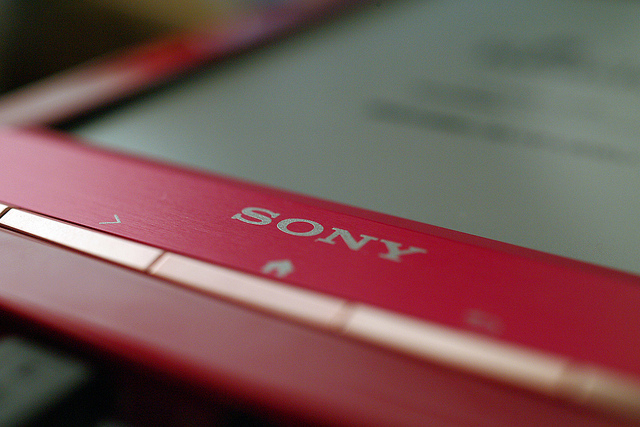
\includegraphics[scale=1]{prs-t1.png}
\end{figure}}$
  \tableofcontents
\end{frame}

\begin{frame}
  \frametitle{Un Ebook-reader}
  Avantages d'un lecteur d'ebook sur une bibliothèque:
  \begin{itemize}
    \pause \item portable, léger;
    \pause \item autonomie (trois semaines à un mois, lecture d'epub);
    \pause \item économique/écologique (papier généralement créee à partir d'arbres);
    \pause \item prise de notes non destructive;
    \pause \item partage de fichiers;
    \item etc.
  \end{itemize}
\end{frame}

\begin{frame}
  \frametitle{Problématique}
  Pas de format standard pour la gestion des notes sur un
  ebook quelconque.
  Les notes sont stockés sur le lecteur:
  \begin{itemize}
    \pause \item à moitié dans une base de données SQLite;
    \pause \item à moitié dans des fichiers XML.
  \end{itemize}

\end{frame}

\end{document}
